\documentclass[pdf]{beamer}
\mode<presentation>{\usetheme{Warsaw}}

%List of packages
\usepackage{graphicx}
\usepackage{caption}
\usepackage{subcaption}
\usepackage[utf8]{inputenc}
\usepackage{amsmath}
\usepackage[version=4]{mhchem}

%%%%%%%%%%%
% Metadata
%%%%%%%%%%%

\hypersetup
{
	%Separate multiple authors by comma
    pdfauthor={Gustavo Estrela,
                Marcelo S. Reis},
	pdftitle={Model Selection for Cell Signaling Pathways},
	pdfsubject={Master's Degree Dissertation},
	pdfkeywords={parameter estimation, ODE, model selection, SPSAS19},
	colorlinks=false
}

%%%%%%%%%%%%%%%%
% Title related
%%%%%%%%%%%%%%%%

\setbeamertemplate{subsection in toc}[default]

%The contact for one of the authors MUST be embedded on the title (see below)
\title[Contact: Gustavo Estela (gestrela@ime.usp.br)]{Model Selection for Cell Signaling Pathways}

%For LICENSE, we suggest CC-BY-SA, but you are free to choose your own as long
%as the LICENSE you choose is AT LEAST as permissive as CC-BY-SA
\author[Gustavo Estrela, Marcelo S. Reis \hspace{0.2cm} {\includegraphics[height=0.2cm, keepaspectratio]{8015.png}}]
{\texorpdfstring{Student: Gustavo Estrela \\ Supervisor: Marcelo S. Reis}{}}

\date[2019]{SPSAS - 2019}

\institute{Institute of Mathematics and Statistics - University of São 
            Paulo (IME-USP).\\
           Special Laboratory of Cell Cycle, Butantan Institute.\\
\tiny{During the development of this work, the author received financial
support from São Paulo Research Foundation (FAPESP).}}

%%%%%%%%%%%%%%%%%%%%%%%%%%%
% Presentation begins here
%%%%%%%%%%%%%%%%%%%%%%%%%%%

\begin{document}

\begin{frame}
	\titlepage
\end{frame}


\begin{frame}
\frametitle{Cell Signaling}
\begin{figure}
	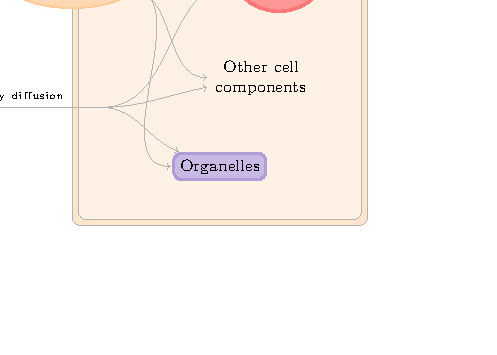
\includegraphics[width=.8\linewidth]{img/introduction/signaling_mechanism.pdf}
\end{figure}
\end{frame}

\begin{frame}
\frametitle{Cell Signaling Pathways}
\begin{figure}
\includegraphics[width=.8\linewidth]{img/experiments/diagrams/smallest_model4.pdf}
\end{figure}
These structures models change of concentrations of proteins.
\end{frame}

\begin{frame}
\frametitle{Ranking Models}
\begin{itemize}
    \item{Define a likelihood function $p ({\bf D} | M, {\bf \theta})$.}
    \pause
    \item{Marginalize it to obtain $p ({\bf D} | M)$.
    \begin{equation*}
        p ({\bf D} | M) = \int_{\Theta} p ({\bf D} | M, {\bf \theta}) 
            p ({\bf \theta} | M) d{\bf \theta},
    \end{equation*}
}
\end{itemize}
\end{frame}

\begin{frame}
\frametitle{Proposing Models}
\begin{itemize}
    \item{Gather possible interactions from databases such as KEGG and
        STRING;}
    \pause
    \item{Systematically remove/add these chemical reactions to a model
        to create new models.}
\end{itemize}
\end{frame}
\end{document}
